\section{Test}

%Lav mindst tre testcases med tilhørende fremgangsmåde/testprocedure og testrapporter.
%Lav mindst én Junit test til centrale metoder. Inkludér code coverage dokumentation.
%Lav mindst én brugertest. Husk at brugeren skal være en der ikke kan kode.




\subsection{Brugertest}

\subsection{Programtest}
Vi har lavet tre JUnit tests af vores version af matadorspillet. Testene tester hhv. terningens tilfældighed, chancekortene tilfældighed samt test af antallet af chancekortene.

\subsubsection{Test af terningens tilfældighed}
    \begin{figure}[H]
        \centering
        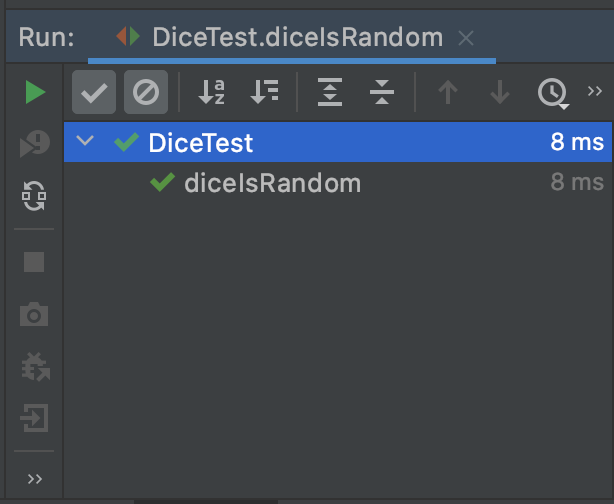
\includegraphics[width=8cm]{figures/diceIsRandomTest.png}
        \caption{JUnit test for at teste tilfældigheden af Dice klassens metode roll()}
        \emph{Testen af Dice klassen og dens roll() metode var en succes. Koden ses i bilag \ref{diceTest}}
    \end{figure}
    Testen af Dice klassen gør brug af et for loop, som køres 100.000 gange. I loopet gør vi brug af Dice klassens roll() metode, for at kaste med terningen. Vi tjekker hver slag, for at se om man slog 1. Efter loopet og de 100.000 slag med terningen, tjekker vi om vi har slået 1 med terningen det forventede antal gange. Vi tester altså om antallet af gange 1 blev slået, afviger væsentligt fra det forvende antal. Gør den det, fejler testen.
    

\subsubsection{Test af chancekort tilfældighed}
    \begin{figure}[H]
        \centering
        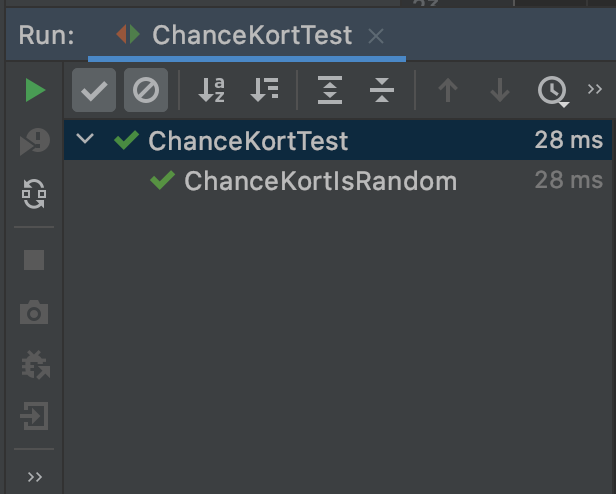
\includegraphics[width=8cm]{figures/chanceKortIsRandom.png}
        \caption{JUnit test for at teste tilfældigheden af ChanceKort klassens metode randomChanceKort()}
        \emph{Testen af ChanceKort klassen og dens randomChanceKort() metode var en succes. Koden ses i bilag \ref{ChanceKortTest}}
    \end{figure}
    Testen her er opbygget på samme måde som testen af Dice klassens tilfældighed. Vi kører randomChanceKort() metoden 100.000 gange og ser om vi fik kort 1 færre eller flere gange end forventet. Denne test er lavet da alle 24 kort var med i spillet, hvilket senere er blevet ændret. For at testen skal have succes, skal der derfor tilføjet alle 24 kort metoder igen. 
    
    
\subsubsection{Test af antal chancekort}
    \begin{figure}[H]
        \centering
        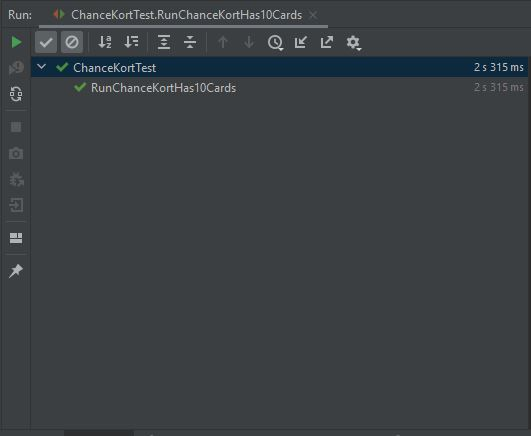
\includegraphics[width=15cm]{figures/RunChanceKortHas10Cards.JPG}
        \caption{JUnit test for at teste at RunChanceKort klassen indeholder det rigtige antal kort.}
        \emph{Testen af RunChanceKort klassen var en succes. Koden ses i bilag \ref{ChanceKortTest}}
    \end{figure}
    Vi har her ændret antal chance kort til 10 i stedet for 24. Her tester vi så antallet af kort, for at sikre at det kun er de 10 kort der er med i spillet. Det gør vi ved at oprette et array med alle de forskellige metoder i RunChanceKort klassen. Vi husker at der er 12 metoder (10 kort() metoder og 2 andre private metoder, som bruges i kort() metoderne). Til sidst sammenligner vi længden af arrayet med det forventede antal ved brug af assertEquals(expected, actual);


\subsubsection{Coverage dokumentation}
\begin{figure}[H]
        \centering
        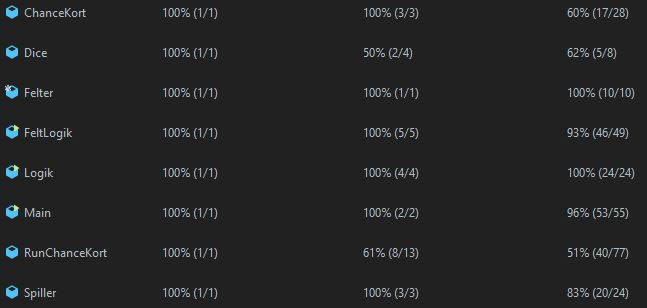
\includegraphics[width=15cm]{figures/codeCoverage.JPG}
        \caption{Code Coverage test}
        \emph{Resultaternes rækkefølge fra venstre til højre er hhv. klasse, metoder og linjer}
    \end{figure}
    Ud over JUnit testene har vi lavet en Code Coverage test, som tester hvor meget af den skrevne kode bliver kørt, når programmet bliver spillet.
    Som resultat af testen bliver alle klasser og 78\% af alle linjer brugt. Dette kan dog variere fra gang til gang, da bl.a. antallet af brugte chancekort ændrer sig. RunChanceKort er derfor den eneste klasse, hvor det vil variere hvor mange af klassens metoder, der vil blive brugt. Da de forskellige chancekort sjældent bliver brugt, har vi valgt, at lave en JUnit test netop til chancekortene så vi ved, at alle chancekort har mulighed for at blive kørt.
    
    \begin{figure}[H]
        \centering
        
\includegraphics[width=12cm]{figures/diceCoverage.JPG}
        \caption{JUnit Dice Coverage test}
        \emph{Resultaternes rækkefølge fra venstre til højre er hhv. klasse, metoder og linjer}
    \end{figure}
    
    \begin{figure}[H]
        \centering
        
\includegraphics[width=12cm]{figures/chanceCoverage.JPG}
        \caption{JUnit ChanceKort Coverage test}
        \emph{Resultaternes rækkefølge fra venstre til højre er hhv. klasse, metoder og linjer}
    \end{figure}

I de to ovenstående figurer er vist Code Coverage ved hhv. DiceTest og ChanceKortTest. Kun 2/4 af metoderne i Dice og 2/3 af metoderne i ChanceKort bliver kørt ved denne test, da de restende metoder ikke er nødvendige for at køre testen. Testen tager ikke brug af disse metoder, da de ikke er nødvendige for vores program.

